\chapter{Analysis} \label{chap:analysis}

\section{Common Attack Scenarios}

Here is a list of common phishing attacks and how \namesecureworkstation/ defends against such attacks.

\subsection{Attacks via email}

\paragraph{Scenario:} The first attack is a popular phishing email attack \cite{attack-verify-email}. The user receives an email appearing to come from Microsoft. It claims that unless the user ``verifies" their account, their account may be closed down. The link to verify leads to a fake sign in page tricking the users to enter their credentials. Figure \ref{fig:attack-verify-email} shows an example of such a phishing email.

\paragraph{Currently:} If the user overlooks the source of the email address (which is onmicrosoft.com) and the URL of the fake sign in page, their credentials will be stolen by the attacker.

\paragraph{Quboid:} Clicking on the verify link opens up a new browser instance with an unrecognized domain name. The interface warns the users that this page has an unrecognized domain. The top area also displays the site-aggregate name of the web page not being Microsoft. The user looks at these cues and recognizes that the web page is a phishing page. However, if the user does not recognize these cues, their credentials may still get stolen by the attacker.

\afterpage{\clearpage}
\begin{figure}[p]
\centering
    \fbox{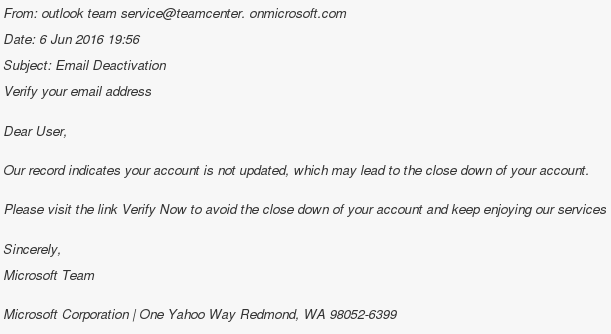
\includegraphics[width=1.0\textwidth]{attack-verify-email.png}}
    \caption{This phishing email appears to come from Microsoft but the domain is suspicious (onmicrosoft.com). The verify link contained in the email leads the user to a fake login page.}
   \label{fig:attack-verify-email}
\end{figure}

\paragraph{Similar Attacks:} There are several other attacks that work in similar ways as to this attack \cite{attack-verify-email-1}\cite{attack-verify-email-2}\cite{attack-verify-email-3}. All these emails start out with a threat of having the user's account closed and asks the user to enter their credentials on a fake login page.

\noindent\rule[0.5ex]{\linewidth}{1pt}

\paragraph{Scenario:} A majority of phishing emails aim at delivering ransomwares to the users. A report by PhishMe estimates that over 97\% of phishing emails deliver ransomwares. The user receives an email asking them to open an attachment which contains information of a delivery as a ZIP file. The attachment contains a ransomware executable. Figure~\ref{fig:attack-ransomware} shows an example of such an email.

\paragraph{Currently:} Upon opening, the ransomware starts executing and encrypts the user's hard disk.

\paragraph{Quboid:} The attachment opens in a new isolated virtual machine since the link belonged to a different site-aggregate. Even though the ransomware is able to execute, it does no damage since it can access only the contents of the isolated virtual machine. It also doesn't have access to data from other browser instances since they run in separate virtual machines. This prevents the malicious software to steal data associated with logged in sessions on other websites.

\begin{figure}[p]
\centering
    \fbox{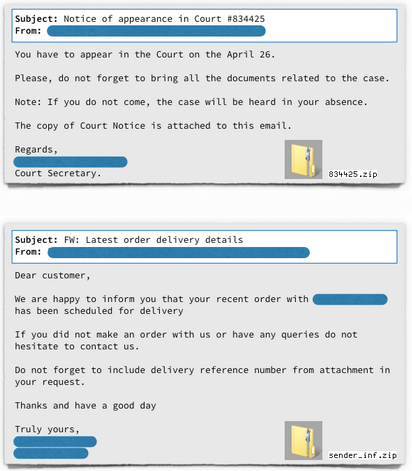
\includegraphics[width=1.0\textwidth]{attack-ransomware-email.png}}
    \caption{This phishing email appears to contain legitimate content but instead contains a ransomware in the attached ZIP file.}
   \label{fig:attack-ransomware}
\end{figure}

\paragraph{Similar Attacks:} A variant of this attack is a phishing email which doesn't actually has any attachment but has an image which appears to be an attachment. To an unsuspecting user, it appears to be a legitimate attachment and he/she expects that the attachment has already been scanned for malware by the email client. However, the attachment image is actually a link that redirects to a page that downloads the malware.

\subsection{Malvertisements}

Malvertisements is another way in which phishing attacks can occur. The internet economy is based on online advertisements. Large websites offer ad spaces by directly contacting target companies. Small scale websites, on the other hand, use intermediate advertising services in order to display ads. If one of these intermediate services gets compromised, all other websites that use that service may get compromised as well. Specifically, consider the following scenario:

\paragraph{Scenario:} The user is browsing a website which uses an external advertisement provider. The provider's system was compromised and the attacker has uploaded a malicious advertisement. For example, if a bank website is displaying an advertisement, the advertisement might claim to be a credit card sign-up form and ask the user for their social security number.

\paragraph{Currently:} The user thinks that it is a genuine form and submits their details to the attacker's server. The attacker can then steal the information entered in the form.

\paragraph{Quboid:} Although the user might enter their details into the fake form, since the bank website does not list the attacker's server as an allowed exit destination, the browser is forbidden from communicating any information to the server. Clicking on the link will just open a new browser instance with the submit URL of the form without any form data being submitted along with the request. This mechanism only works if the external advertisement does not include malicious Javascript. For example, most email client block any Javascript from executing in HTML emails. A malicious script may be able to encode the form data in other ways, thus defeating the purpose of controlling the exit URLs.

\paragraph{Similar Attacks:} Similarly, the advertisement can display a link to fake login page. However, if that link belongs to a different site-aggregate, the URL will open in a separate browser instance and the interface will clearly show the site-aggregate name of the new web page.

\subsection{Attacks using User Interface Ambiguity}

\paragraph{Scenario:} While visiting a website, a popup appears which looks like the Chrome prompt. The prompt says that the user's computer is infected with a virus and an antivirus software must be downloaded. The software downloaded is actually a malware.

\paragraph{Currently:} The popup appears indistinguishable from the actual system prompt to an unsuspecting user. The user downloads the infected software.

\paragraph{Quboid:} The user expects system prompts to be displayed only in the reserved area. Hence, there is a higher chance of the user suspecting something is wrong if any system-prompt looking content is displayed in the application content area.

% \noindent\rule[0.5ex]{\linewidth}{1pt}

% \paragraph{Scenario:} You get an email saying you need to ``verify" your account, else it will be deactivated. There is a link in the email that points to a webpage which asks you to enter your password.

% \paragraph{Currently:} You get an email saying you need to ``verify" your account, else it will be deactivated. There is a link in the email that points to a webpage which asks you to enter your password.

% \paragraph{Solution:} You get an email saying you need to ``verify" your account, else it will be deactivated. There is a link in the email that points to a webpage which asks you to enter your password.

% \noindent\rule[0.5ex]{\linewidth}{1pt}

% \paragraph{Scenario:} You get an email saying you need to ``verify" your account, else it will be deactivated. There is a link in the email that points to a webpage which asks you to enter your password.

% \paragraph{Currently:} You get an email saying you need to ``verify" your account, else it will be deactivated. There is a link in the email that points to a webpage which asks you to enter your password.

% \paragraph{Solution:} You get an email saying you need to ``verify" your account, else it will be deactivated. There is a link in the email that points to a webpage which asks you to enter your password.

% \noindent\rule[0.5ex]{\linewidth}{1pt}

% \paragraph{Scenario:} You get an email saying you need to ``verify" your account, else it will be deactivated. There is a link in the email that points to a webpage which asks you to enter your password.

% \paragraph{Currently:} You get an email saying you need to ``verify" your account, else it will be deactivated. There is a link in the email that points to a webpage which asks you to enter your password.

% \paragraph{Solution:} You get an email saying you need to ``verify" your account, else it will be deactivated. There is a link in the email that points to a webpage which asks you to enter your password.

% \noindent\rule[0.5ex]{\linewidth}{1pt}

% \paragraph{Scenario:} You get an email saying you need to ``verify" your account, else it will be deactivated. There is a link in the email that points to a webpage which asks you to enter your password.

% \paragraph{Currently:} You get an email saying you need to ``verify" your account, else it will be deactivated. There is a link in the email that points to a webpage which asks you to enter your password.

% \paragraph{Solution:} You get an email saying you need to ``verify" your account, else it will be deactivated. There is a link in the email that points to a webpage which asks you to enter your password.

% \noindent\rule[0.5ex]{\linewidth}{1pt}

\subsection{Other Attacks}

\paragraph{Scenario:} An attacker is able to poison the DNS resolver cache of the user's local system. The new entries point to the attackers server where a fake login page is displayed.

\paragraph{Currently:} The user believes the fake login page to be genuine and enters their credentials. The attacker can not steal these credentials.

\paragraph{Quboid:} Since the DNS resolver cache is poisoned, it fails DNSSEC integrity checks. The proxy VM blocks the request from going through in the first place.

\noindent\rule[0.5ex]{\linewidth}{1pt}

\paragraph{Scenario:} An attacker may be using a man-in-the-middle server to sniff all the content that the user is browsing. In the usual case, any traffic that has been encrypted using SSL/TLS should not be visible to the attacker. However, if the attacker is able to obtain a fake certificate for a website which was issued by a trusted CA, the man-in-the-middle server may be able to sniff the encrypted traffic to that website as well.

\paragraph{Currently:} If the fake certificate was issued by a trusted CA, there is no way the user can identify that such an attack is taking place.

\paragraph{Quboid:} The DNS records for the website also contains DANE entries. These entries have the public the key of the certificate that the website uses. Since the keys in the DNS record and the keys in the certificate presented by the attacker will not match up, the system will reject the request and notify the user that the DANE validation failed.

% \begin{itemize}
%     \item  You get an email saying you need to “verify” your account otherwise it will be deactivated. The link goes to a link that asks for your password.

%     \item Poisoning DNS caches to redirect common websites to attackers versions.

%     \item Lured victims into entering their dropbox credentials on a page hosted on dropbox itself. Similarly, for any other websites which let you host content. http://www.csoonline.com/article/2953190/vulnerabilities/google-drive-phishing-is-back-with-obfuscation.html http://www.symantec.com/connect/blogs/dropbox-users-targeted-phishing-scam-hosted-dropbox

%     \item Email stating someone sent you a Google Doc. You open it, and it leads to a OAuth authorization page stating the app needs access. You click yes, the page redirects to an external attackers link with an authorized token.

%     \item RSA security keys were stolen when a flash vulnerability was used in a spear phishing attack.

%     \item Nigerian Prince scam wire money to this account/dating website email

%     \item Malicious Email with a malicious email attachment.

%     \item Placed phishing content on a legitimate server of some org. E.g. paypal login on srilankan government page

%     \item Go to a website, popup comes says download a software in order to access something. It is a malicious software

%     \item Popup comes saying you have a problem with your computer, call number to connect to a tech support service.

%     \item We have recieved a password reset request, please go to this webpage and enter your old password.

%     \item A post on a legitimate website e.g. Airbnb requesting to circumvent the website’s payment procedure and use an external service e.g. western union. You may get an email saying the same with a scam email address.

%     \item Fake online surveys which may ask for personal information

%     \item Tracking notification for UPS containing a malicious exe

%     \item Online websites which send you fake goods

%     \item Facebook fake friend

%     \item Tax services scams

%     \item Credentials stolen on Steam. Attackers can put arbitrary javascript code in their profile. Can be used to redirect users to some other page, steal login cookie.

%     \item Link is a data:text/html url containing a whole login page. The link is disguised as an attachment.

%     \item Lastpass users tricked into entering their credentials on a fake lastpass page.

%     \item Puny code lets you get https certs for a fake domain which appears as real domain on your browser

%     \item M.facebook.com---------------------------------.stuff

%     \item Blockhain.com

%     \item Search engine phishing/credit card offers - give up personally identifiable information

%     \item Sometimes legit sites don’t include ownership information in their SSL certificates. Additionally they may use multiple domains. Impossible to identify right from wrong. Either verify the website externally, or SRP like password.

%     \item LetsEncrypt makes Chrome show “Secure” on the URL bar. Anyone can create certs.
% \end{itemize}

\subsection{Attacks that Quboid does not defend against}

Quboid provides several mechanism to make the user aware that a phishing attack may be taking place. However, it is still possible for the user to overlook these cues. In these cases, Quboid does not prevent against the effects resulting from these attacks.

\paragraph{Scenario:} The user unknowingly visits a malicious site which has a pop-up notifying that their computer may have a virus and they need to call the given phone number in order to request tech support. If the user fails to notice that this prompt was not generated by the system, they continue with the call and may potentially reveal sensitive information. Since this is a completely offline attack, our system cannot defend against this attack.

\paragraph{Scenario:} If the user fails to notice the site-aggregate name of a website being displayed in the top reserved area, it is possible for a phishing attack to still succeed by displaying fake login pages. Although Quboid provide several cues, an uncareful user may be able to miss them.

\section{Quboid Defense Mechanisms}

Quboid employs several defense mechanisms as we saw in earlier chapters. Here we list these defense mechanisms and explain the attack scenarios that they prevent:

\paragraph{Separate VM's:} Each browser instance runs in a separate VM. In the event that the user executes a malicious downloaded file, the damage remains contained within that virtual machine.

\paragraph{Site Aggregates:} Websites forming a single unit are grouped together in a single site-aggregate. Phishing websites which pretend to be other website will not be part of this aggregate and Quboid will display this information.

\paragraph{Proxy Filter:} All network traffic is routed through an intermediate proxy. The proxy ensures that a virtual machine can access content only from its own site-aggregate, even in the event that the virtual machine has itself been compromised.

\paragraph{Exit URL Whitelist:} A whitelist is contained in the HTTP response headers which lists the URLs that a page is allowed to submit form data to. This is helpful in case the browser displays external HTML-only content where the external content has been compromised. It prevents data being submitted outside of the site-aggregate of the browser.

\paragraph{External Resources Whitelist:} The external resources whitelist allows sites to retrieve content from external websites but prevents the browsers from navigating directly to these websites.

\paragraph{Secure User Interface:} The user interface of Quboid is separated into two: application and system. This prevents attacks where a website may try to fake a system prompt and lead the user into downloading malicious software.

\section{Implementation Overhead}

\subsection{Network Latency}

All network traffic is routed through a proxy VM. This results in an increased latency during web browsing. We measured this latency by first measuring the latency when requesting a web page without going through a proxy, and then measuring the latency with the proxy. We used \texttt{mitmproxy}, a Python based proxy, for our measurements and implementation.

Figure~\ref{fig:latency} lists the average latency measured in three different scenarios: (1) without a proxy VM, (2) through a proxy without any filter rules, and (3) through a proxy with filter rules.

\begin{figure}
\centering
    \begin{tabular}{| l | l |}
    \hline
    \textbf{Scenario} & \textbf{Latency} \\ \hline
    Without proxy & 15ms $\pm$ 2ms \\ \hline
    With proxy without filter & 28ms $\pm$ 6ms \\ \hline
    With filter proxy & 860ms $\pm$ 7ms \\ \hline
    \hline
    \end{tabular}
\caption{Average latency in different proxy configurations} \label{fig:latency}
\end{figure}

We find that the latency introduced just by adding an intermediate proxy is not significant. However, filter rules adds significant amount of latency. This latency can be reduced by having more efficient implementations of the proxy software and of the filter.

\subsection{Virtualization Overhead}

Although Qubes employs various techniques to speed up virtual machine creation, it still takes some time to start new VMs. We measured the time it takes to open new browser instances in Qubes disposable VMs. We measured the opening times with different number of virtual machines already running on the system. This shows any performance limitations that could arise during the normal browsing experience.

Figure~\ref{fig:openvm} shows a plot of the average time to open new VMs vs. number of existing running VMs. We imagine that in a normal browsing session, the user has around 6-7 web-aggregates open in the VMs. For up to that number of VMs, we do not see any significant performance hit.

$ $\\

\begin{figure}
\centering
\begin{tikzpicture}[y=1cm, x=1cm,font=\sffamily]
 	%axis
	\draw (0,0) -- coordinate (x axis mid) (7,0);
    	\draw (0,0) -- coordinate (y axis mid) (0,6);
    	%ticks
    	\foreach \x in {0,...,7}
     		\draw (\x,1pt) -- (\x,-3pt)
			node[anchor=north] {\x};
    	\foreach \y in {0,...,6}
     		\draw (1pt,\y) -- (-3pt,\y) 
     			node[anchor=east] {\y}; 
	%labels      
	\node[below=0.8cm] at (x axis mid) {\# of existing VMs};
	\node[rotate=90, above=0.8cm] at (y axis mid) {Time to open new VM [s]};

	%plots
	\draw plot[mark=square*]
		file {openvm.data};  
\end{tikzpicture}
\caption{Plot of average VM opening time vs. the number of existing running VMs} \label{fig:openvm}
\end{figure}

\subsection{User Experience}

Quboid changes the browsing experience for the user in a number of ways.

\paragraph{Separate VMs per site-aggregate:} Each site-aggregate is opened in a separate VM. Opening new VMs is slower than opening new tabs in a modern web browser. This is a trade-off that Quboid makes between usability vs. the security offered by virtualization.

\paragraph{Single Application Window Manager:} Quboid diverges from the more popular tiling window managers by using a single application window manager. Only one browser instance may be displayed on the screen at a time. Different browser instances are switched by using the application switching shortcuts in the window manager. This restricts the usability in the event that the user needs to look at content from multiple browser instances at the same time.

\paragraph{Restricting downloads to VMs:} Any application downloaded by the user is run in a separate VM. Thus, it cannot access content from applications running in different VMs. Everyday tasks such as downloading a media player to play movies require extra steps since the user has to now move the movie to the media player VM before playing.
